%%%%%%%%%%%%%%%%%%%%%%%%%%%%%%%%%%%%%%%%%%%%%%%%%%%%%%%%%%%%%%%%%%%%%%%%%%%%%%%%
%2345678901234567890123456789012345678901234567890123456789012345678901234567890
%        1         2         3         4         5         6         7         8

%\documentclass[letterpaper, 10 pt, conference]{ieeeconf}  % Comment this line out if you need a4paper

\documentclass[a4paper, 10pt, conference]{ieeeconf}      % Use this line for a4 paper

\IEEEoverridecommandlockouts                              % This command is only needed if 
                                                          % you want to use the \thanks command

\overrideIEEEmargins                                      % Needed to meet printer requirements.

%In case you encounter the following error:
%Error 1010 The PDF file may be corrupt (unable to open PDF file) OR
%Error 1000 An error occurred while parsing a contents stream. Unable to analyze the PDF file.
%This is a known problem with pdfLaTeX conversion filter. The file cannot be opened with acrobat reader
%Please use one of the alternatives below to circumvent this error by uncommenting one or the other
%\pdfobjcompresslevel=0
%\pdfminorversion=4

% See the \addtolength command later in the file to balance the column lengths
% on the last page of the document

% The following packages can be found on http:\\www.ctan.org
\usepackage{graphicx} % for pdf, bitmapped graphics files
%\usepackage{epsfig} % for postscript graphics files
\usepackage{mathptmx} % assumes new font selection scheme installed
%\usepackage{times} % assumes new font selection scheme installed
\usepackage{amsmath} % assumes amsmath package installed
\usepackage{amssymb}  % assumes amsmath package installed

\title{\LARGE \bf
Generation of Complex Road Networks Using a Simplified Logical Description for the Validation of Automated Vehicles*
}


\author{Daniel Becker$^{1}$ and Lutz Eckstein$^{2}$% <-this % stops a space
\thanks{*This research is funded by the SET Level 4to5 research initiative, promoted by the	Federal Ministry for Economic Affairs and Energy (BMWi).}% <-this % stops a space
\thanks{$^{1}$Daniel Becker is with the automated driving department of the Institute
	for Automotive Engineering (ika), RWTH Aachen University, 52074
	Aachen, Germany {\tt\small daniel.becker@ika.rwth-aachen.de}}%
\thanks{$^{2}$Lutz Eckstein is head of the Institute for Automotive Engineering
	(ika), RWTH Aachen University, 52074 Aachen, Germany {\tt\small lutz.eckstein@ika.rwth-aachen.de}}%
}


\begin{document}


\maketitle
\thispagestyle{empty}
\pagestyle{empty}


%%%%%%%%%%%%%%%%%%%%%%%%%%%%%%%%%%%%%%%%%%%%%%%%%%%%%%%%%%%%%%%%%%%%%%%%%%%%%%%%
\begin{abstract}
The verification and validation of automated driving functions is an essential building block in the process of releasing those functions to the public. 
\end{abstract}


%%%%%%%%%%%%%%%%%%%%%%%%%%%%%%%%%%%%%%%%%%%%%%%%%%%%%%%%%%%%%%%%%%%%%%%%%%%%%%%%
\section{INTRODUCTION}

To assure the safety of automated driving functions (ADF), verification and validation methods need to developed and established. (testfahrten und nötige km. etc erklären. zu Szenarien und simulation überleiten)

One approach to reach this state is scenario based testing. [ref] proposed different stages of scenarios: functional, logical and concrete. The term functional states a linguistic description which allows experts to talk about scenarios at an early stage of the development process. In logical scenarios parameters and ideally their probability distributions are provided. Finally, concrete scenarios specify a distinct value for each parameter which makes them feasible to be executed reproducible in a simulation or on proving grounds. Each stage can be divided into six levels (ref. EN layer ,hendrik) where the three lower layers describe the static part of the scenario, i.e. the road. Layer four focuses on moving objects, whereas layer five and six describe environmental conditions and vehicle-to-everything (V2X) communication, respectively. Detailed discussion in [ref hendrik eindhoven] (oder schreibt man das nicht?)

Current research initiatives such as SET Level 4to5 (footnote?) address simulative scenario based testing with focus on inner city traffic. Besides layer four which describes the dynamic behavior of all participants, the static scenery has to be taken into account as well. The latter is described within layer one to three and has to be defined in a logical and concrete manner, respectively. The open source standard format OpenDRIVE [ref asam] is suitable for concrete descriptions of road networks and is widely used in industry and research. However, by now there is no standardized logical road description format which is easy to use and capable to be transfered into OpenDRIVE. 

This article introduces a prototypical logical description language for complex road networks and a tool which generates concrete, standardized OpenDRIVE maps which may be used for the simulative testing of ADF.

\begin{figure}[thpb] 		
	\centering
	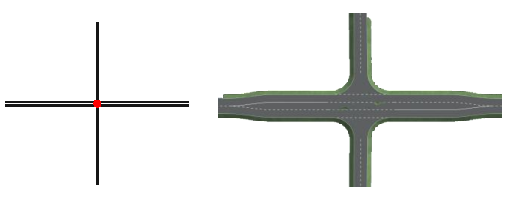
\includegraphics{fig/motivation.pdf}
	\caption{Graphical example of input and output of the road generation tool. As a minimal input two reference lines with assigned road types and a coupling point are sufficient to generate an intersection written in valid OpenDRIVE. (OpenDRIVE visualized in CarMaker 8.0[ref?]) \textbf{roughDraft}}
	\label{fig_curvGraph}
\end{figure}

\section{RELATED WORK}
During the research initiative PEGASUS [ref] these concepts have been developed and utilized within the domain German motorway. Furthermore, the main focus has been on layer four. Nevertheless, when moving the testing domain to inner city scenarios such as the driving behavior on intersections, layers one to three are much more complex. Motorways usually consist of parallel lanes which follow curves with big radii. Such a road is not complicated to describe and generate. It can be done automatically with low effort. [ref. menzel et al.] propose a method to create a standardized road network in the OpenDRIVE format from a logical (and functional) road description. However, inner city intersections are more complex both in the logical description and in terms of the concrete format. 

die Frage ist, was alles "related" ist... eventuell kuerzer halten und laengere introduction?

\section{METHODOLOGY}

\section{LOGICAL ROAD DESCRIPTION}
The proposed logical road description is derived from the reference line concept of OpenDRIVE. This means that each lane is described by an offset from a reference line defined in the x,y-plane (topview). However, in contrast to OpenDRIVE we introduce some simplifications and eliminate redundancies along the reference line. Each road segment consists of the geometric primitives line, arc and spiral, which is motivated by the federal guidelines for road constructions [ref]. In order to ensure a smooth driveability along the road network, we define that the curvature graph has to be continuous. Therefor, the definition of curvature over distance, a start point and initial heading is sufficient to uniquely describe a road segment's course. Fig. \ref{fig_curvGraph} shows the definition of a road segment that is composed of the geometric primitive sequence line-spiral-arc-spiral-line.
\begin{figure}[thpb] 		
	\centering
	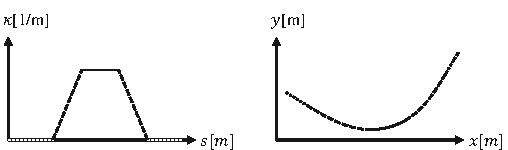
\includegraphics{fig/curvGraph.pdf}
	\caption{Example for a curve defined by the curvature graph. The plan view results from two integrations over $s$. Geometric primitives: line-spiral-arc-spiral-line. Positive curvature values correspond to left turns in positive $s$ direction.\textbf{roughDraft}}
	\label{fig_curvGraph}
\end{figure}

\textit{short introduction to curvature graph integral}

\textit{now explain tree structure}

\begin{figure}[thpb] 		
	\centering
	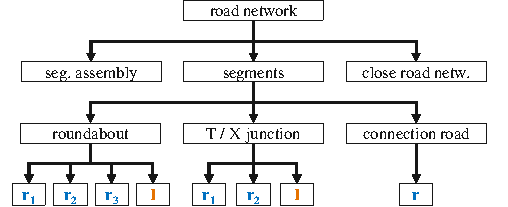
\includegraphics{fig/schema.pdf}
	\caption{Hierarchical structure of the road network. On the first level all segments and their relation to each other are defined. In addition, it is possible to define the automatic connection of two road ends. Segments are defined as roundabouts, junctions and connection roads. $r_i$ and $I$ describe roads and intersection definitions, respectively}
	\label{figurelabel}
\end{figure}
\section{ROAD GENERATION}

\subsection{Geometry}

\subsection{Intersections}

\subsection{Road Network}

\section{RESULTS}

\begin{table}[h]
\caption{An Example of a Table}
\label{table_example}
\begin{center}
\begin{tabular}{|c|c|}
\hline
One & Two\\
\hline
Three & Four\\
\hline
\end{tabular}
\end{center}
\end{table}

\section{CONCLUSIONS}

\addtolength{\textheight}{-12cm}   % This command serves to balance the column lengths
                                  % on the last page of the document manually. It shortens
                                  % the textheight of the last page by a suitable amount.
                                  % This command does not take effect until the next page
                                  % so it should come on the page before the last. Make
                                  % sure that you do not shorten the textheight too much.

%%%%%%%%%%%%%%%%%%%%%%%%%%%%%%%%%%%%%%%%%%%%%%%%%%%%%%%%%%%%%%%%%%%%%%%%%%%%%%%%



%%%%%%%%%%%%%%%%%%%%%%%%%%%%%%%%%%%%%%%%%%%%%%%%%%%%%%%%%%%%%%%%%%%%%%%%%%%%%%%%



%%%%%%%%%%%%%%%%%%%%%%%%%%%%%%%%%%%%%%%%%%%%%%%%%%%%%%%%%%%%%%%%%%%%%%%%%%%%%%%%

\begin{thebibliography}{99}

\bibitem{c1} G. O. Young, Synthetic structure of industrial plastics (Book style with paper title and editor), 	in Plastics, 2nd ed. vol. 3, J. Peters, Ed.  New York: McGraw-Hill, 1964, pp. 15-64.
\bibitem{c2} W.-K. Chen, Linear Networks and Systems (Book style).	Belmont, CA: Wadsworth, 1993, pp. 123-135.


\end{thebibliography}




\end{document}
